\documentclass{article}
\usepackage[margin=1in]{geometry}
\usepackage{amsmath,amsthm,amssymb}
\usepackage{bbm,enumerate,mathtools}
\usepackage{tikz,pgfplots}
\usepackage{chessboard}
\usepackage[hidelinks]{hyperref}
\usepackage{multicol} % Problem 35

\newenvironment{question}{\begin{trivlist}\item[\textbf{Question.}]}{\end{trivlist}}
\newenvironment{note}{\begin{trivlist}\item[\textbf{Note.}]}{\end{trivlist}}
\newenvironment{references}{\begin{trivlist}\item[\textbf{References.}]}{\end{trivlist}}
\newenvironment{related}{\begin{trivlist}\item[\textbf{Related.}]\end{trivlist}\begin{enumerate}}{\end{enumerate}}


\begin{document}
\rating{2}{3}
OEIS sequence A261865 describes ``$a(n)$ is the least $k \in \mathbb{N}$ such
that some multiple of $\sqrt{k} \in (n, n+1)$.'' Clearly the asymptotic
density of $2$ in the sequence is $1/\sqrt{2}$.
\begin{figure}[!h]
  \centering
  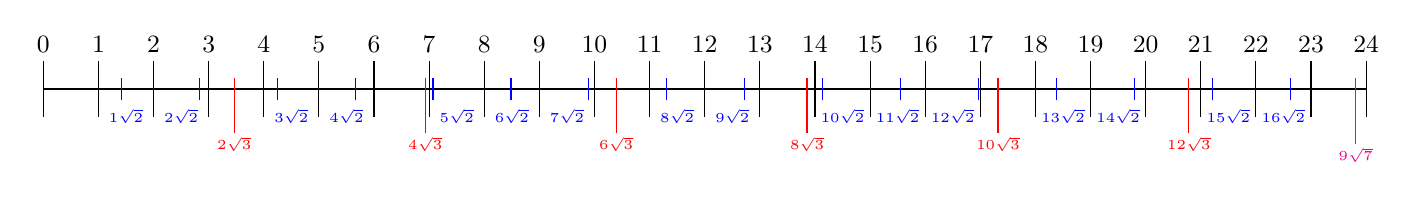
\begin{tikzpicture}[scale=0.7]
    \draw (0,0.5) -- (24,0.5);
    \foreach \x in {0,...,24} {
      \node at (\x, 1.3) {\small$\x$};
      \draw (\x,0)--(\x,1);
    }

    \foreach \x in {1,...,16} {
      \draw[blue] (1.41421 * \x,0.3)--(1.41421 * \x,0.7);
      \node[blue] at ({floor(1.41421 * \x) + 0.5}, 0) {\tiny$\x\sqrt{2}$};
    }

    \foreach \x in {2,4,6,8,10,12} {
      \draw[red] ({sqrt(3) * \x},-0.3)--({sqrt(3) * \x},0.7);
      \node[red] at ({sqrt(3) * \x}, -0.5) {\tiny$\x\sqrt{3}$};
    }

    \foreach \x in {9} {
      \draw[magenta] ({sqrt(7) * \x},-0.5)--({sqrt(7) * \x},0.7);
      \node[magenta] at ({sqrt(7) * \x}, -0.7) {\tiny$\x\sqrt{7}$};
    }
  \end{tikzpicture}
  \caption{
    An illustration of $a(n)$ for $n \in \{1,2,\hdots,23\}$.
  }
\end{figure}

\begin{question}
  Let $S_\alpha \subset \mathbb{N}$ denote the squarefree integers strictly
  less than $\alpha$.\\
  Is the asymptotic density of squarefree $j$ given by \[
    \frac{1}{\sqrt{j}}\prod_{s \in S_j}\left(1 - \frac{1}{\sqrt{s}}\right)?
  \]
\end{question}

\begin{related}
  \item Is there an algorithm to construct a value of $n$ such that $a(n) > K$
    for any specified $K$?
    (Perhaps using best Diophantine approximations or something?)
  \item What is the asymptotic growth of the records?
  \item Given some $\alpha$ what is the expected value of the smallest $n$ such
    that $S_\alpha \subset \{a(1), \hdots, a(n)\}$?
  \item This sequence uses the ``base sequence'' of
    $\{\sqrt{1},\sqrt{2},\sqrt{3},\hdots\}$. On what other base sequences is
    this construction interesting?
  \item What is the smallest $m \in \mathbb{N}$ such that
    $k2^{1/m} \in (n, n+1)$ for some $k \in \mathbb{N}$?
    \item What is the smallest $k \in \mathbb{N}$ such that
      $k2^{1/m} \in (n, n+1)$ for some $m \in \mathbb{N}$?
\end{related}
\begin{references}
  \item \url{https://oeis.org/A261865}
\end{references}
\end{document}
